
%%%%%%%%%%%%%%%%%%%%%%%%%%%%%%%%%%%%%%%%%%%%%%%%%%%%%%%%%%%%%%%%%%%%%%%%%%%%%%%%%%%%%%%
%%%%%%%%%%%%%%%%%%%%%%%%%%%%%%%%%%%%%%%%%%%%%%%%%%%%%%%%%%%%%%%%%%%%%%%%%%%%%%%%%%%%%%%
% 
% This top part of the document is called the 'preamble'.  Modify it with caution!
%
% The real document starts below where it says 'The main document starts here'.

\documentclass[12pt]{article}
\usepackage{hyperref}

\usepackage{amssymb,amsmath,amsthm}
\usepackage[top=1in, bottom=1in, left=1.25in, right=1.25in]{geometry}
\usepackage{fancyhdr}
\usepackage{enumerate}
\usepackage{listings}
\usepackage{graphicx}
\usepackage{float}
\usepackage{multicol}
% Comment the following line to use TeX's default font of Computer Modern.
\usepackage{times,txfonts}
\usepackage{mwe}
\usepackage{caption}
\usepackage{subcaption}

\usepackage{tikz}
\def\checkmark{\tikz\fill[scale=0.4](0,.35) -- (.25,0) -- (1,.7) -- (.25,.15) -- cycle;} 



\makeatletter
\renewcommand*\env@matrix[1][*\c@MaxMatrixCols c]{%
  \hskip -\arraycolsep
  \let\@ifnextchar\new@ifnextchar
  \array{#1}}
\makeatother

\newtheoremstyle{homework}% name of the style to be used
  {18pt}% measure of space to leave above the theorem. E.g.: 3pt
  {12pt}% measure of space to leave below the theorem. E.g.: 3pt
  {}% name of font to use in the body of the theorem
  {}% measure of space to indent
  {\bfseries}% name of head font
  {:}% punctuation between head and body
  {2ex}% space after theorem head; " " = normal interword space
  {}% Manually specify head
\theoremstyle{homework} 

% Set up an Exercise environment and a Solution label.
\newtheorem*{exercisecore}{\@currentlabel}
\newenvironment{exercise}[1]
{\def\@currentlabel{#1}\exercisecore}
{\endexercisecore}

\newcommand{\localhead}[1]{\par\smallskip\noindent\textbf{#1}\nobreak\\}%
\newcommand\solution{\localhead{Solution:}}

%%%%%%%%%%%%%%%%%%%%%%%%%%%%%%%%%%%%%%%%%%%%%%%%%%%%%%%%%%%%%%%%%%%%%%%%
%
% Stuff for getting the name/document date/title across the header
\makeatletter
\RequirePackage{fancyhdr}
\pagestyle{fancy}
\fancyfoot[C]{\ifnum \value{page} > 1\relax\thepage\fi}
\fancyhead[L]{\ifx\@doclabel\@empty\else\@doclabel\fi}
\fancyhead[C]{\ifx\@docdate\@empty\else\@docdate\fi}
\fancyhead[R]{\ifx\@docauthor\@empty\else\@docauthor\fi}
\headheight 15pt

\def\doclabel#1{\gdef\@doclabel{#1}}
\doclabel{Use {\tt\textbackslash doclabel\{MY LABEL\}}.}
\def\docdate#1{\gdef\@docdate{#1}}
\docdate{Use {\tt\textbackslash docdate\{MY DATE\}}.}
\def\docauthor#1{\gdef\@docauthor{#1}}
\docauthor{Use {\tt\textbackslash docauthor\{MY NAME\}}.}
\makeatother

% Shortcuts for blackboard bold number sets (reals, integers, etc.)
\newcommand{\Reals}{\ensuremath{\mathbb R}}
\newcommand{\Nats}{\ensuremath{\mathbb N}}
\newcommand{\Ints}{\ensuremath{\mathbb Z}}
\newcommand{\Rats}{\ensuremath{\mathbb Q}}
\newcommand{\Cplx}{\ensuremath{\mathbb C}}
%% Some equivalents that some people may prefer.
\let\RR\Reals
\let\NN\Nats
\let\II\Ints
\let\CC\Cplx

%\textbf{Code:}
%\begin{center}
%  \lstinputlisting{NewtonsMethodP5.m}
%\end{center}
%
%\textbf{Console:}
%\begin{center}
%  \lstinputlisting{P5C.txt}
%\end{center}
%\vspace{.15in}


%\begin{figure}[H]
%  \begin{center}
%    \caption{The one-norm unit ball}
%    \includegraphics[width=.76\textwidth]{1norm.png}
%  \end{center}
%\end{figure}




%%%%%%%%%%%%%%%%%%%%%%%%%%%%%%%%%%%%%%%%%%%%%%%%%%%%%%%%%%%%%%%%%%%%%%%%%%%%%%%%%%%%%%%
%%%%%%%%%%%%%%%%%%%%%%%%%%%%%%%%%%%%%%%%%%%%%%%%%%%%%%%%%%%%%%%%%%%%%%%%%%%%%%%%%%%%%%%
% 
% The main document start here.

% The following commands set up the material that appears in the header.
\doclabel{Math 615: Homework 6}
\docauthor{Stefano Fochesatto}
\docdate{\today}


\begin{document}


\begin{exercise}{Problem P27}
  \begin{enumerate}
    \item[\textbf{a.}] In preparation for the problem \textbf{P29} below, write two solvers, 
    \begin{equation*}
      \text{function [tt, zz] = feuler(f, eta, t0, tf, N)}
    \end{equation*}
    \begin{equation*}
      \text{function [tt, zz] = rk4(f, eta, t0, tf, N)}
    \end{equation*}
    which imploement schemes $(5.19)$ and $(5.33)$, respectively, to solve the ODE IVP in
    $(5.1)$ and $(5.2)$. The first input to these solver is function $z = f(t, u)$. The other inputs 
    are a vector of initial values $eta = u(t_0)$, the initial time $t0$, the final time $tf$, and the number 
    of equal-length steps $N$. Each solver outputs the entire trajectory, so $tt$ is a 1D array of length $N+1$
    starting with $t_0$ and ending with $t_f$. If $\eta \in \RR^s$ then $zz$ is a 2D array with $s$ rows and $N + 1$
    columns; each column $i$ gives the solution $u(t)$ at the $i$th time $tt$. 
    \solution Consider the following code, 

    \textbf{Code:}
    \begin{center}
      \lstinputlisting[basicstyle = \footnotesize ]{feuler.txt}
    \end{center}



    \textbf{Code:}
    \begin{center}
      \lstinputlisting[basicstyle = \footnotesize ]{rk4.txt}
    \end{center}







    \item[\textbf{b.}] Solve the following simple problem exactly:
    \begin{equation*}
      u''(t) + u(t) = 0 \qquad u(0) = 1,\qquad u'(0) = 0
    \end{equation*}
    \solution
    Clearly the solution is $u(t) = \cos(t)$, here is the solution worked out in detail. First we form the characteristic polynomial by substituting $u(t) = e^{rt}$,
    \begin{align*}
      u''(t) + u(t) &= 0,\\
      r^2e^{rt} + e^{rt} &= 0,\\
      e^{rt}(r^2 + 1) &= 0.
    \end{align*}

    Since our characteristic polynomial has a roots $r = \pm i$ we form the general solution with, 
    \begin{equation*}
      u(t) = c_1e^{it} + c_2e^{-it}. 
    \end{equation*}
    Applying Euler's formula we get a solution of the form, 
    \begin{equation*}
      u(t) = c_1(\cos(t) + i\sin(t)) + c_2(\cos(t) - i\sin(t)).
    \end{equation*}
    Computing the derivative we get, 
    \begin{equation*}
      u'(t) = c_1(-\sin(t) + i\cos(t)) + c_2(-\sin(t) - i\cos(t)).
    \end{equation*}
    Applying our initial values we get, 
    \begin{align*}
      u(0) = 1 &=  c_1(\cos(0) + i\sin(0)) + c_2(\cos(0) - i\sin(0)),\\
        1 &=  c_1 + c_2,\\
    \end{align*}
    and, 
    \begin{align*}
      u'(0)= 0 &= c_1(-\sin(0) + i\cos(0)) + c_2(-\sin(0) - i\cos(0)),\\
      0&= c_1i - c_2i.
    \end{align*}
    Which gives us $c_1 = c_2 = 1/2$, so $u(t) = \cos(t)$ as expected. 


    \item[\textbf{c.}] The problem in $\textbf{b}$, for example on the interval $[0, 2]$, 
    makes a good test case. Demonstrate that the final time numerical error of each solver in $\textbf{a}$
    converges at the expected rate as the timestep $k \to 0$. 
    \solution First we need to rewrite our second order problem as a system of first order equations of the form $u'(t) = f(t, u(t))$. 
    Let $x(t) = u_1(t)$ and $x'(t) = u_2(t)$ and therefore we get the, 
    \begin{align*}
      u'_1(t) &= u_2(t)\\
      u'_2(t) &= -u_1(t)
    \end{align*}
    So as a system with initial conditions $\eta$ we get, 
    \begin{equation*}
      \begin{bmatrix}
        u'_1(t)\\
        u'_2(t)
      \end{bmatrix} = 
      \begin{bmatrix}
        0 & 1\\
        -1 & 0
      \end{bmatrix}
      \begin{bmatrix}
        u_1(t)\\
        u_2(t)
      \end{bmatrix}
    \end{equation*}
    \begin{equation*}
      \eta = \begin{bmatrix}
        1\\
        0
      \end{bmatrix}
    \end{equation*}
    Running this example using our two solvers we get the following convergence rates, $\approx O(k^1)$ for forward euler and $\approx O(k^4)$ for 
    the fourth order Runge Kutta. This is as expected as each each step accumulates a truncation error of $O(k^2)$ for forward euler, after $k$ steps 
    the truncation error is $O(k)$. Similarly with RK4 which accumulates a truncation error of $O(k^5)$ at each step. 

    \begin{figure}[H]
      \begin{center}
        \caption{feuler on test case}
        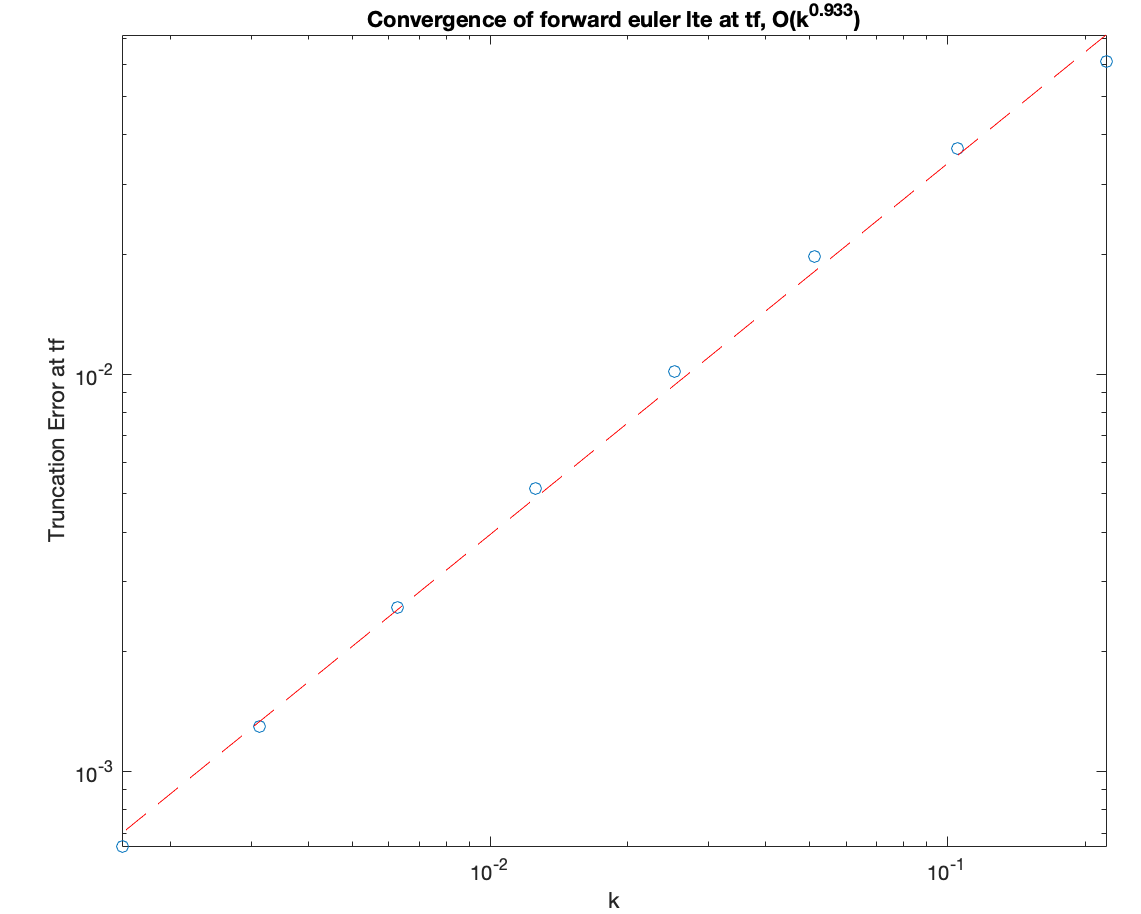
\includegraphics[width=.76\textwidth]{FEConvergence.png}
      \end{center}
    \end{figure}

    \begin{figure}[H]
      \begin{center}
        \caption{rk4 on test case}
        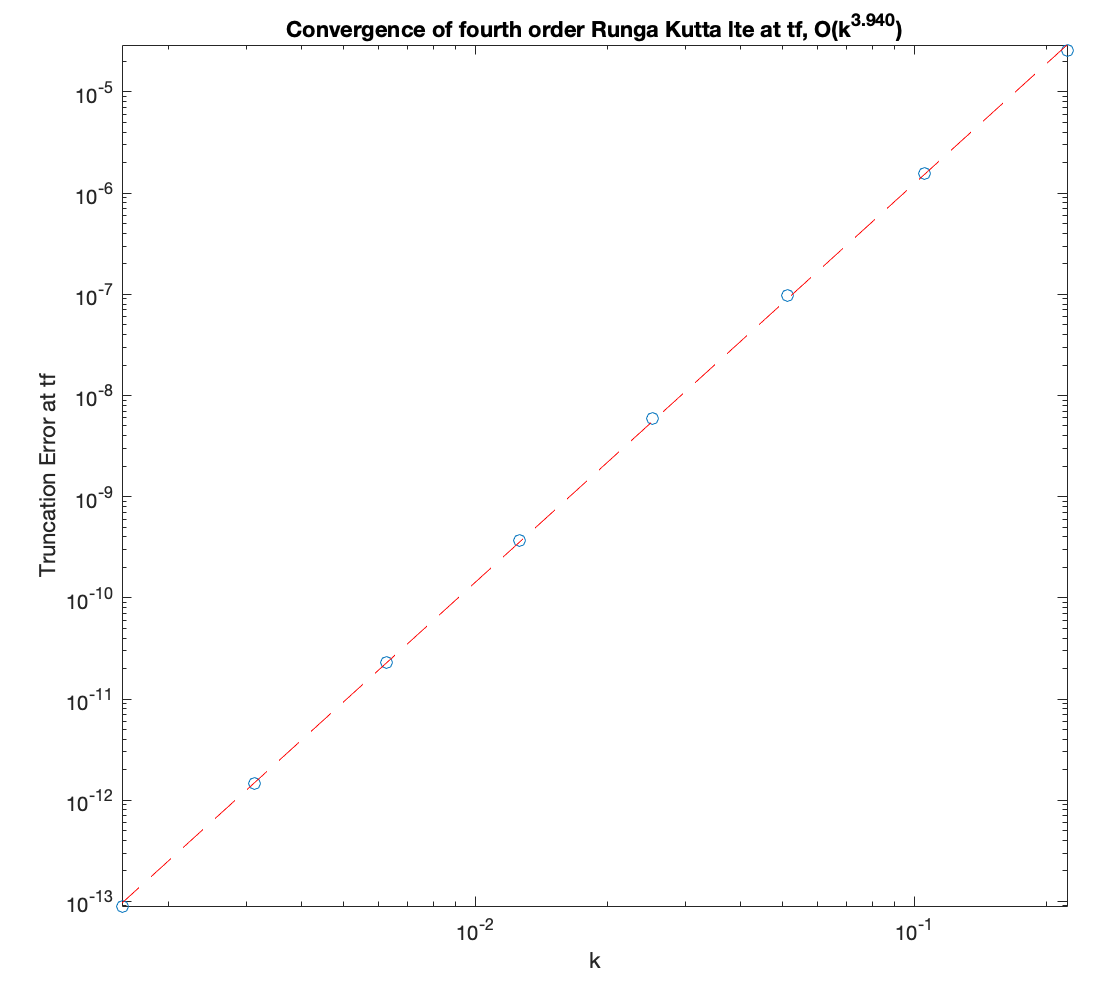
\includegraphics[width=.76\textwidth]{rk4convergence.png}
      \end{center}
    \end{figure}

    \textbf{Code:}
    \begin{center}
      \lstinputlisting[basicstyle = \footnotesize ]{r1.txt}
    \end{center}    
  \end{enumerate} 
\end{exercise}




\begin{exercise}{Problem P28} Compute the leading term in the local truncation error of the following methods. For parts $(\textbf{a})$ and 
  $(\textbf{b})$, please follow the style of Example 5.9, wherein you learn the coefficient of the leading order term. For part $(\textbf{c})$
  you can follow the style of Example 5.11 and only get the order, without knowing the leading order coefficient. 
  \begin{enumerate}
    \item[\textbf{a}] The 2-step BDF method (5.25)
    \solution Recall that the 2-step backwards differentiation method is given by, 
    \begin{equation*}
      \dfrac{3U^{n + 1}-4U^n + U^{n - 1}}{2k} = f(U^{n+1}).
    \end{equation*}
    Computing the truncation error as the residual of the scheme applied to the exact solution, we get, 
    \begin{equation*}
      \tau^{n+1} = \dfrac{3u(t_{n + 1})-4u(t_n) + u(t_{n - 1})}{2k} - f(u({t_{n+1}})).
    \end{equation*}
    Expanding via Taylor's Theorem about $t_{n + 1}$ and substituting the solution $f(u({t_{n+1}})) = u'(t_{n+1})$ we get, 
    \begin{align*}
      \tau^{n+1} &= \dfrac{3u(t_{n + 1})-4u(t_n) + u(t_{n - 1})}{2k} - f(u({t_{n+1}})),\\
      = \dfrac{1}{2k}\biggl(3u(t_{n + 1}) - &4\left(u(t_{n+1}) - ku'(t_{n+1}) + \frac{1}{2}k^2u''(t_{n+1}) - \frac{1}{6}k^3u'''(t_{n+1}) + O(k^4) \right)\\
                  +&\left(u(t_{n+1}) - 2ku'(t_{n+1}) + 2k^2u''(t_{n+1}) - \frac{8}{6}k^3u'''(t_{n+1}) + O(k^4)\right)\biggr) - u'(t_{n+1}),\\
                  =& \dfrac{1}{2k}\biggl(2ku'(t_{n+1}) -\frac{4}{6}k^3u'''(t_{n+1}) + O(k^4)\biggr)- u'(t_{n+1})\\
                  =&-\frac{1}{3}k^2u'''(t_{n+1}) + O(k^3)\\
    \end{align*}


    \item[\textbf{b}] The trapezoidal method (5.22),
    \solution Recall that the trapezoidal method is given by, 
    \begin{equation*}
      \dfrac{U^{n+1} - U^n}{k} = \frac{1}{2}(f(U^n) + f(U^{n+1})).
    \end{equation*}
    Computing the truncation error $\tau^*$ for the $\tau_n + \frac{1}{2}k$ term,  
    \begin{equation*}
      \tau^* = \dfrac{u(t_{n+1})-u(t_{n})}{k} - \frac{1}{2}(f(u(t_{n})) + f(u(t_{n+1})))
    \end{equation*}
    Expanding via Taylor's Theorem about $t_* = t_n + \frac{1}{2}k$ and substituting the solution $f(u({t_{n+1}})) = u'(t_{n+1})$ and $f(u({t_{n}})) = u'(t_{n})$,
    \begin{align*}
      \tau^* = \dfrac{1}{k}  \biggl(&\left(u(t_*) + \frac{1}{2}ku'(t_{*}) + \frac{1}{8}k^2u''(t_{*}) + \frac{1}{48}k^3u'''(t_{*}) + O(k^4)\right)\\
      - &\left(u(t_*) - \frac{1}{2}ku'(t_{*}) + \frac{1}{8}k^2u''(t_{*}) - \frac{1}{48}k^3u'''(t_{*}) + O(k^4)\right)\biggr)\\
      - &\dfrac{1}{2}\left(u'(t_{n}) + u'(t_{n + 1})\right),\\
    \end{align*}
    \begin{align*}
      \tau^* = \dfrac{1}{k}  \biggl(&\left(u(t_*) + \frac{1}{2}ku'(t_{*}) + \frac{1}{8}k^2u''(t_{*}) + \frac{1}{48}k^3u'''(t_{*}) + O(k^4)\right)\\
      - &\left(u(t_*) - \frac{1}{2}ku'(t_{*}) + \frac{1}{8}k^2u''(t_{*}) - \frac{1}{48}k^3u'''(t_{*}) + O(k^4)\right)\biggr)\\
      - \dfrac{1}{2}  \biggl(&\left(u'(t_{*}) - \frac{1}{2}ku''(t_{*}) + \frac{1}{8}k^2u'''(t_{*}) - \frac{1}{48}k^3u''''(t_{*}) + O(k^4)\right)\\
      + &\left( u'(t_{*}) + \frac{1}{2}ku''(t_{*}) + \frac{1}{8}k^2u'''(t_{*}) + \frac{1}{48}k^3u''''(t_{*}) + O(k^4)\right)\biggr),\\
    \end{align*}

    \begin{align*}
      \tau^* = \dfrac{1}{k}&\left(  ku'(t_{*})+\frac{1}{24}k^3u'''(t_{*}) + O(k^4)\right)\\
      - \dfrac{1}{2}&\left(2u'(t_{*}) + \frac{1}{4}k^2u'''(t_{*}) + O(k^4)\right),\\
      &=-\frac{1}{12}k^2u'''(t_{*}) + O(k^4).
    \end{align*}

    \item[\textbf{c}] The explicit trapezoid method, 
    \begin{equation*}
      U^{n+1} = U^n + \frac{k}{2}\biggl(f(U^n) + f\biggl(U^n + kf(U^n)\biggr)\biggr).
    \end{equation*}
    \solution Computing the truncation error we get the following, 
    \begin{equation*}
      \tau^n = \frac{1}{k} \left(u(t_{n+1}) - u(t_n)\right) - \frac{1}{2}\biggl(f(u(t_n)) + f\biggl(u(t_n) + kf(u(t_n))\biggr)\biggr).
    \end{equation*}
    Note that by substitution of the exact solution, 
    \begin{equation*}
      f\biggl(u(t_n) + kf(u(t_n))\biggr) =  f\biggl(u(t_n) + ku'(t_n)\biggr).
    \end{equation*}
    Expanding the function via Taylor's Theorem about $u(t_n)$, and substituting the exact solution and $f'(u)u' = u''$ , 
    \begin{align*}
      f\biggl(u(t_n) + ku'(t_n)\biggr) &= f(u(t_n)) + ku'(t_n)f'(u(t_n)) + \frac{1}{2}k^2(u'(t_n))^2f''(u(t_n)) + \dots \\
      &= u'(t_n) + ku''(t_n) + O(k^2).
    \end{align*}
    Substituting into our original truncation error calculation, and using Taylor's Theorem to expand $u(t_{n+1})$ about $t_n$ we get, 
    \begin{align*}
      \tau^n &= \frac{1}{k} \left(u(t_{n+1}) - u(t_n)\right) - \frac{1}{2}\biggl(f(u(t_n)) + f\biggl(u(t_n) + kf(u(t_n))\biggr)\biggr),\\
      &=\frac{1}{k}\biggl(u(t_n) + ku'(t_n) + \frac{1}{2}k^2u''(t_n) + \frac{1}{6}k^3u'''(t_n) + O(k^4) - u(t_n)\biggr) \\
      &- \frac{1}{2}(u'(t_n)) - \frac{1}{2} \biggl( u'(t_n) + ku''(t_n) + O(k^2)\biggr),\\
      &= u'(t_n) + \frac{1}{2}ku''(t_n) + \frac{1}{6}k^2u'''(t_n) + O(k^3) - \frac{1}{2}(u'(t_n)) - \frac{1}{2}\biggl( u'(t_n) + ku''(t_n) + O(k^2)\biggr),\\
      &= O(k^2).
    \end{align*}
  \end{enumerate} 
  
\end{exercise}


\begin{exercise}{Problem P29} Consider the problem of two massive bodies, with masses $m_1$, 
  and $m_2$. They are attracted by gravity only. They travel in a plane so their positions are 
  given by vector-values functions $x_i(t) = (x_i(t), y_i(t))$ for $i = 1, 2$. Newton's second 
  law and Newton's law of gravity combine to say:
  \begin{equation*}
    m_1x''_1 = -Gm_1m_2\frac{x_1 - x_2}{|x_1 - x_2|^3}
  \end{equation*}
  \begin{equation*}
    m_2x''_2 = -Gm_1m_2\frac{x_2 - x_1}{|x_1 - x_2|^3}
  \end{equation*}
  We will consider the Earch and the Moon in isolation as our example. Thus the 
  constants are, 
  \begin{equation*}
    m_1 = 5.972 \times 10^{24} kg
  \end{equation*}
  \begin{equation*}
    m_2 = 7.348 \times 10^{22} kg
  \end{equation*}
  \begin{equation*}
    G = 6.674 \times 10^{-11} m^3kg^{-1}s^{-2}
  \end{equation*}
  and we measure $t$ in seconds and $x_i,y_i$ in meters. 
  
  \begin{enumerate}
    \item[\textbf{a}] By using notation $v_i = x'_i$, $w_i = y'_i$ for $i = 1, 2$, write 
    the problem as a first oder ODE system of dimension $s = 8$, with solution column vector $u(t) \in \RR^8$. 
    Use the component ordering,
    \begin{align*}
      u(t) &= [x_1(t) \qquad y_1(t) \qquad x_2(t) \qquad y_2(t)\qquad v_1(t) \qquad w_1(t) \qquad v_2(t) \qquad w_2(t)]^T\\
        &= [u_1(t) \qquad u_2(t) \qquad u_3(t) \qquad u_4(t) \qquad u_5(t) \qquad u_6(t) \qquad u_7(t) \qquad u_8(t)]^T
    \end{align*}
    That is, write the system in the form $u'(t) = f(t, u(t))$. Then implement a single function, 
    \begin{equation*}
      \text{ function z = fearthmoon(t, u)}
    \end{equation*}
    which compute the right-hand-side function $f(t, u)$ of the ODE system. 
  
  \solution Rewriting the system in the form of $u'(t) = f(t, u(t))$ with the given substitution, 
  \begin{align*}
    u'(t) &= [x'_1(t) \qquad y'_1(t) \qquad x'_2(t) \qquad y'_2(t)\qquad v'_1(t) \qquad w'_1(t) \qquad v'_2(t) \qquad w'_2(t)]^T\\
    = [&v_1(t) \quad w_1(t) \quad v_2(t) \quad w_2(t)\quad \\
    &-Gm_2\frac{x_1(t) - x_2(t)}{|x_1 - x_2|^3} \quad -Gm_2\frac{y_1(t) - y_2(t)}{|x_1 - x_2|^3} \quad -Gm_1\frac{x_2(t) - x_1(t)}{|x_1 - x_2|^3} \quad -Gm_1\frac{y_2(t) - y_1(t)}{|x_1 - x_2|^3}]^T\\
    = [&u_5(t) \quad u_6(t) \quad u_7(t) \quad u_8(t)\quad \\
    &-Gm_2\frac{u_1(t) - u_3(t)}{|x_1 - x_2|^3} \quad -Gm_2\frac{u_2(t) - u_4(t)}{|x_1 - x_2|^3} \quad -Gm_1\frac{u_3(t) - u_1(t)}{|x_1 - x_2|^3} \quad -Gm_1\frac{u_4(t) - u_2(t)}{|x_1 - x_2|^3}]^T
  \end{align*}
  Finally let $|x_1 - x_2|^3 = \left(\sqrt{(u_1(t) - u_3(t))^2 + (u_2(t) - u_4(t))^2}\right)^{3}$.

  \item[\textbf{b}]
  \solution 
  The following is a code for the matlab function fearthmoon(t, u), \\

  \textbf{Code:}
    \begin{center}
      \lstinputlisting[basicstyle = \footnotesize ]{t2.txt}
    \end{center}    

    The following are the figures produced by solving the system using rk4, feuler, and ode45, as well as the driver code for generating 
    the figures, 
    \begin{figure}[H]
      \begin{center}
        \caption{feuler solution for $N = 40$}
        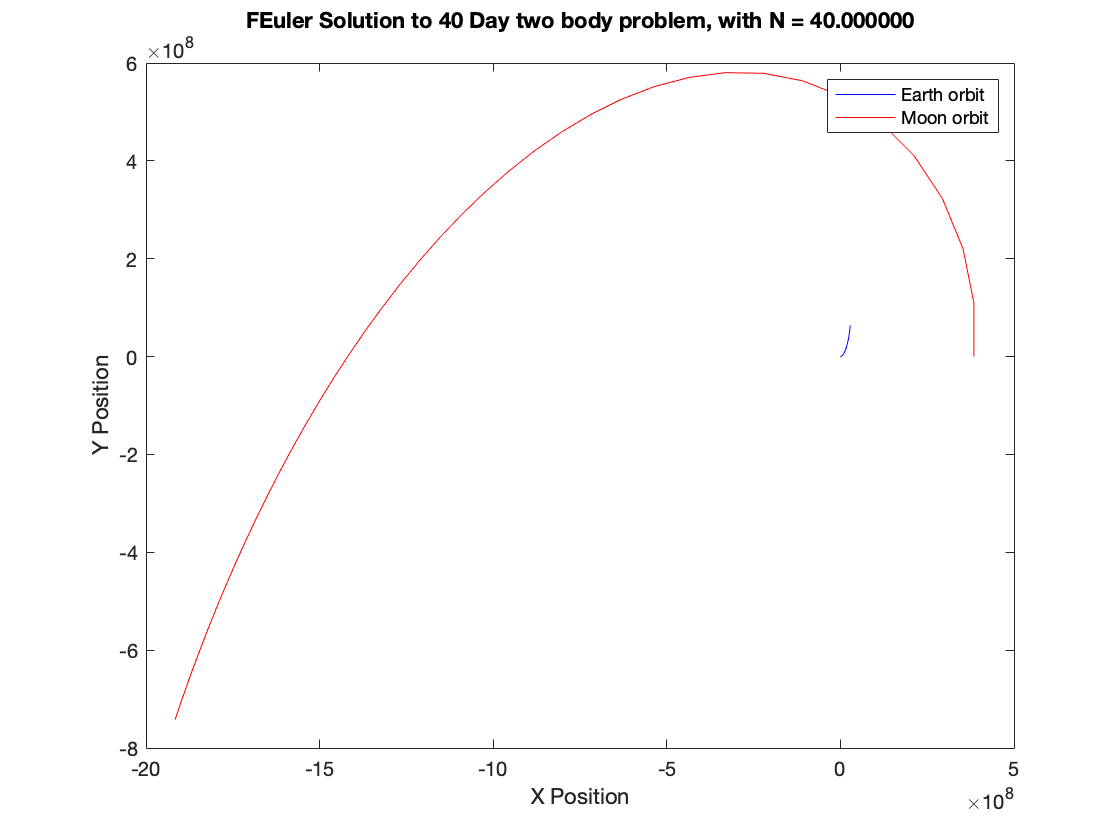
\includegraphics[width=\textwidth]{FEulerN40.png}
      \end{center}
    \end{figure}

    \begin{figure}[H]
      \begin{center}
        \caption{feuler solution for $N = 960$}
        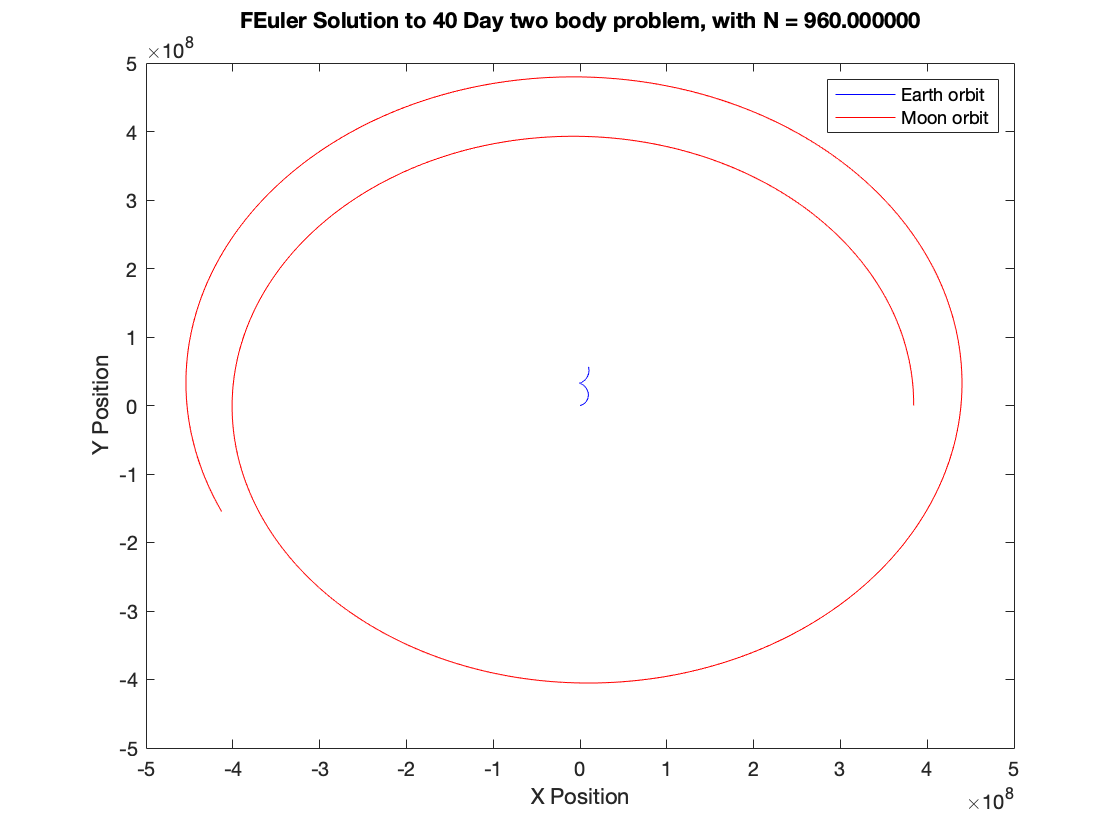
\includegraphics[width=\textwidth]{FEulerN960.png}
      \end{center}
    \end{figure}

    \begin{figure}[H]
      \begin{center}
        \caption{rk4 solution for $N = 40$}
        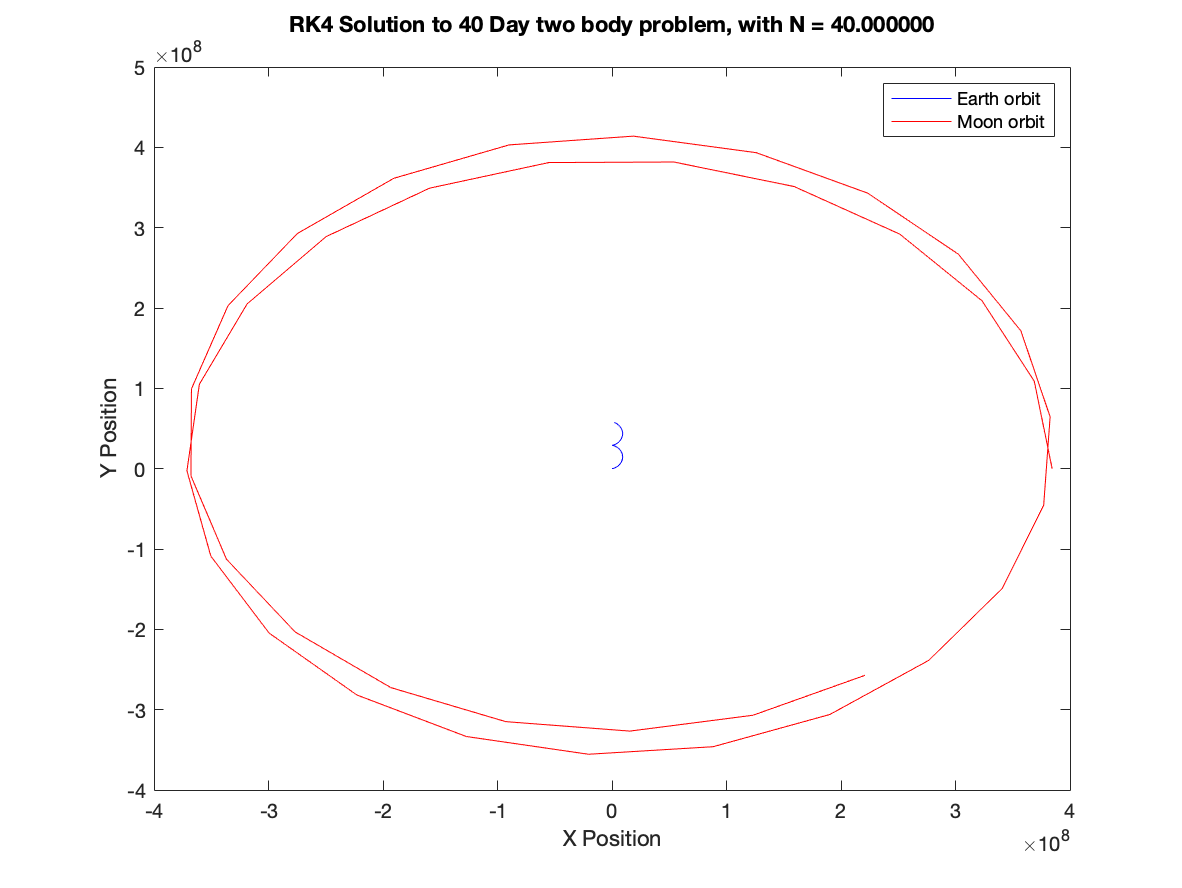
\includegraphics[width=\textwidth]{RK4N40.png}
      \end{center}
    \end{figure}

    \begin{figure}[H]
      \begin{center}
        \caption{rk4 solution for $N = 960$}
        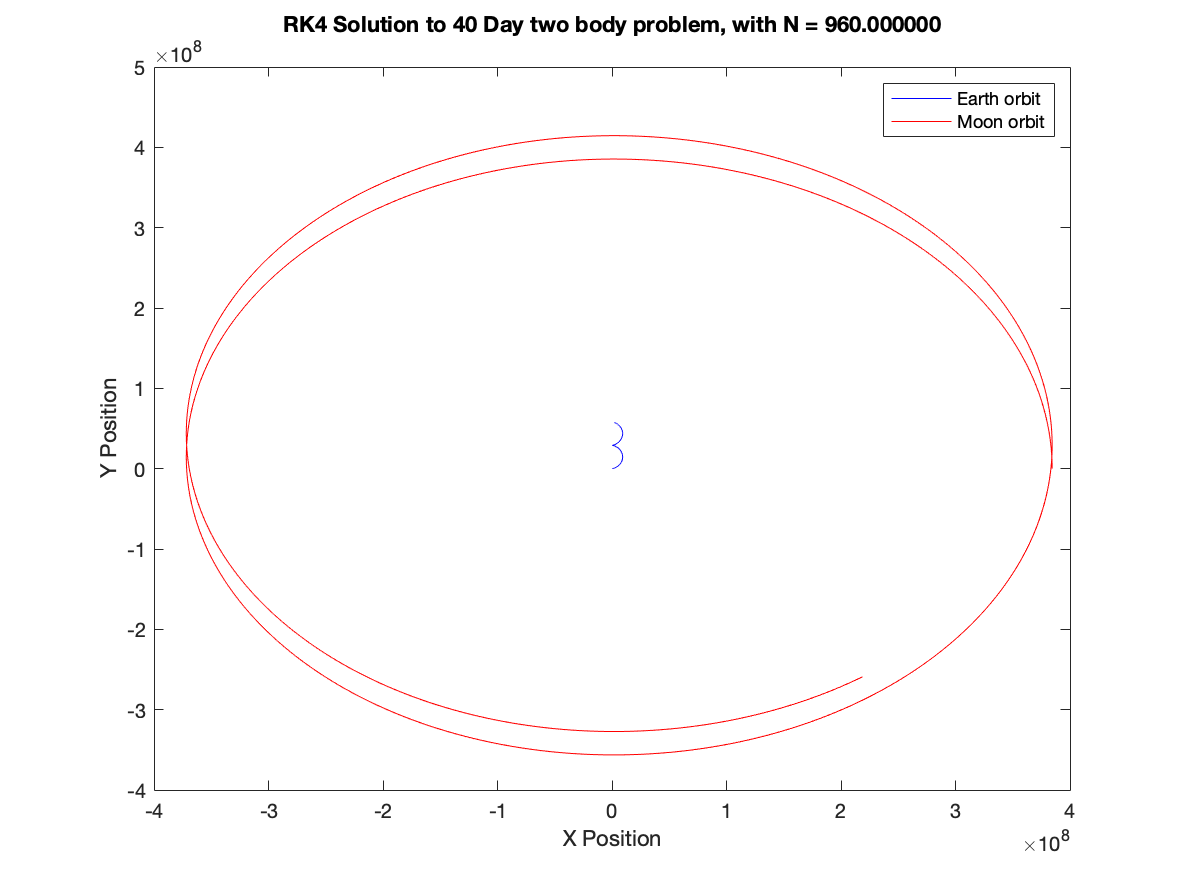
\includegraphics[width=\textwidth]{RK4N960.png}
      \end{center}
    \end{figure}

    \begin{figure}[H]
      \begin{center}
        \caption{ode45 solution for default step sizes}
        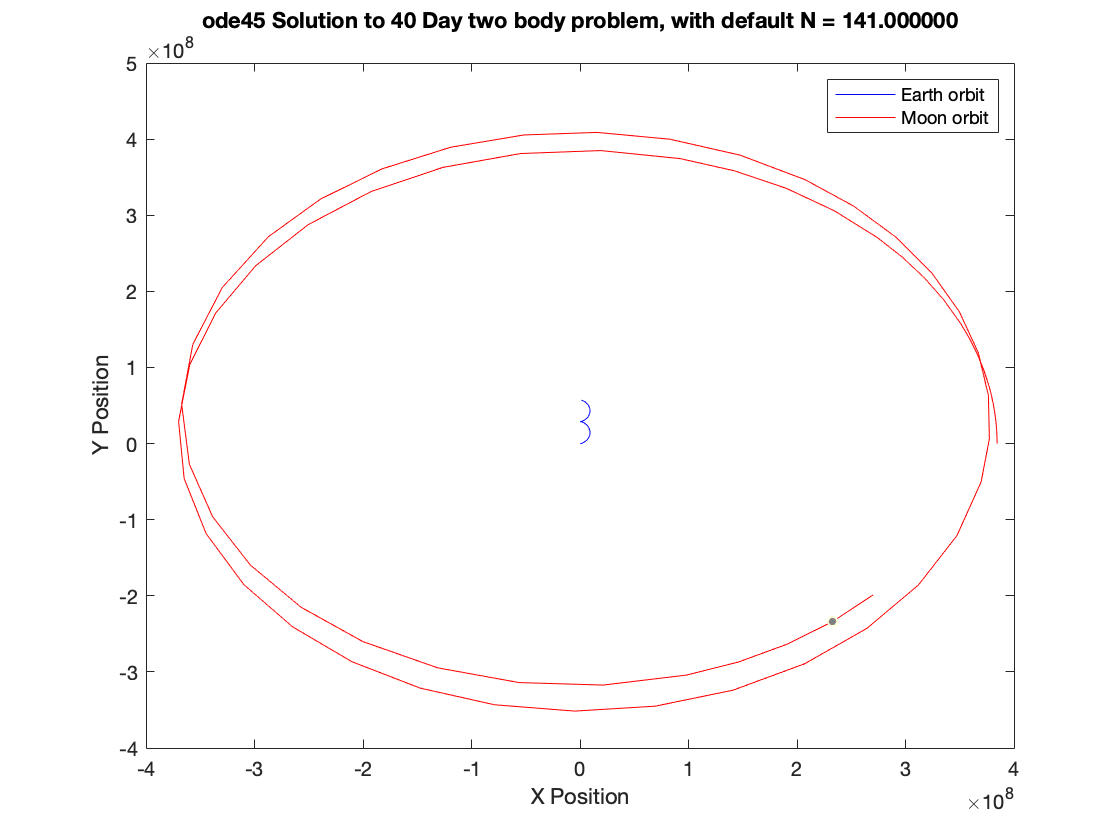
\includegraphics[width=\textwidth]{ODE45NDefault.png}
      \end{center}
    \end{figure}

    \textbf{Code:}
    \begin{center}
      \lstinputlisting[basicstyle = \footnotesize ]{r3.txt}
    \end{center}    


    \item[\textbf{c}] How long is a lunar month, if we used your computations in part \textbf{b}
    \solution Consider the following matlab code, which computes the normalized difference vector between
    the moon position and earth position to get a relative moon orbit. Then we choose the first position
    and innerproduct that with the rest of the relative moon orbit, taking the maximum index to see which time step
    achieves the same position. It computes to approx 21 days which I certain is incorrect, and I'm not sure if it's a bug in the code 
    or the calculation. \\

    \textbf{Code:}
    \begin{center}
      \lstinputlisting[basicstyle = \footnotesize ]{r4.txt}
    \end{center}    



  \end{enumerate}

  
\end{exercise}















\end{document}











 




